\documentclass[12pt]{article}
\usepackage{graphicx,multicol,mdwlist}
\usepackage{charter,amsmath,amssymb,breakurl}
\usepackage{eulervm}
\usepackage[letterpaper,margin=1in]{geometry}
\title{Math 265 Quiz 4}\author{}\date{}
\let\cos\relax\DeclareMathOperator{\cos}{\mathsf{cos}}
\let\ln\relax\DeclareMathOperator{\ln}{\mathsf{ln}}
\everymath{\displaystyle}
\begin{document}
\maketitle
\thispagestyle{empty}
\begin{multicols}{2}
Consider the vector field $\mathbold{F}\left(x,y\right)
=\left\langle 3y,-3x\right\rangle$, which is shown
at the right, together with the curve $C$,
which consists of a semicircle centered at the origin
between $\left(-1,1\right)$ and $\left(1,-1\right)$,
joined to a line segment with the same endpoints.
$C$ is oriented counterclockwise.
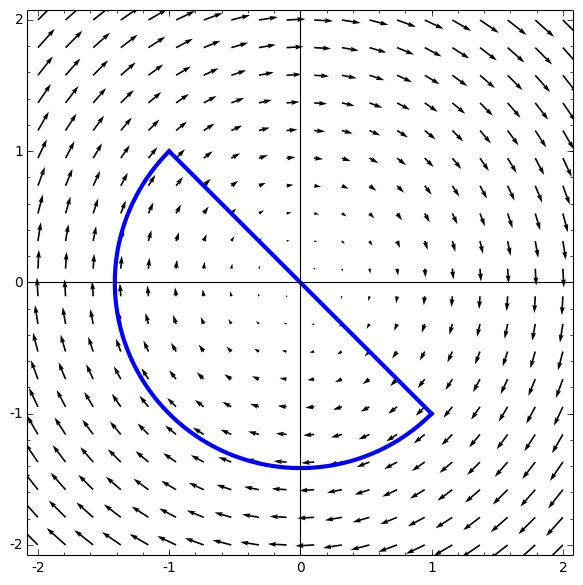
\includegraphics[scale=.6]{Cardioid}
\end{multicols}
\begin{enumerate}
\item Is $\mathbold{F}$ conservative?
\vspace{1in}
\item Calculate the circulation $\oint_C\mathbold{F}
\cdot d\mathbold{r}$ directly.
\vspace{2in}
\item Calculate the circulation $\oint_C\mathbold{F}
\cdot d\mathbold{r}$ using Green's Theorem.
\vspace{4in}
\item Calculate the outward flux $\oint_C\mathbold{F}
\cdot\mathbold{n}\;ds$ using Green's Theorem.
\end{enumerate}
\end{document}
